\documentclass[a4paper,12pt]{article}
\usepackage[utf8]{inputenc}
\usepackage[spanish]{babel}
\usepackage{color}
\usepackage{parskip}
\usepackage{graphicx}
\usepackage{multirow}
\usepackage{listings}
\usepackage{vmargin}
\usepackage{datetime}
\newdate{date}{28}{12}{2017}
\graphicspath{ {imagenes/} }
\definecolor{mygreen}{rgb}{0,0.6,0}
\definecolor{lbcolor}{rgb}{0.9,0.9,0.9}
\usepackage{epstopdf}
\usepackage{float}


\setpapersize{A4}
\setmargins{2.5cm}       % margen izquierdo
{1.5cm}                        % margen superior
{16.5cm}                      % anchura del texto
{23.42cm}                    % altura del texto
{10pt}                           % altura de los encabezados
{1cm}                           % espacio entre el texto y los encabezados
{0pt}                             % altura del pie de página
{2cm}     

\lstset{
    tabsize=4,    
%   rulecolor=,
    language=[GNU]C++,
        basicstyle=\tiny,
        aboveskip={1.5\baselineskip},
        columns=fixed,
        showstringspaces=false,
        extendedchars=false,
        breaklines=true,
        prebreak = \raisebox{0ex}[0ex][0ex]{\ensuremath{\hookleftarrow}},
        frame=single,
        showtabs=false,
        showspaces=false,
        showstringspaces=false,
        identifierstyle=\ttfamily,
        keywordstyle=\color[rgb]{0,0,1},
        commentstyle=\color[rgb]{0.026,0.112,0.095},
        stringstyle=\color{red},
        numberstyle=\color[rgb]{0.205, 0.142, 0.73},
%        \lstdefinestyle{C++}{language=C++,style=numbers}’.
}


\begin{document}
\title{Proyecto Final}
\author{
Christofer Fabián Chávez Carazas \\
\small{Universidad Nacional de San Agustín de Arequipa} \\
\small{Escuela Profesional de Ciencia de la Computación} \\
\small{Compiladores}
}
\date{\displaydate{date}}

\maketitle

\begin{enumerate}
 \item \textbf{Enunciado}
 
 Construir un compilador que reconozca funcionalidades básicas del lenguaje C.
 
 \item \textbf{Herramientas}
 
 Para construir el compilador se utilizaron las siguientes herramientas:
 \begin{itemize}
  \item Lex, para construir el analizador léxico.
  \item Yacc, para construir el analizador sintáctico y semántico.
 \end{itemize}
 
 \item \textbf{Código}
 
 El código está escrito en dos archivos: ``lexico.l'' y ``sintactico.y''
 
 \begin{enumerate}
  \item \textbf{lexico.l}
  
  Aquí se encuentra el analizador léxico del programa escrito en Lex. En el código se muestra un listado de las expresiones regulares y los tokens que
  el analizador léxico reconoce y luego envía al analizador sintáctico.
  
  \begin{lstlisting}
%{
	#include "y.h"
	#include <stdlib.h>
	#include <stdio.h>
%}



%option yylineno
lineComm \/\/.*\n
white [ \t\r\f\n]+
integer [0-9]+
floating [0-9]+\.[0-9]+
real [+-][0-9]+\.[0-9]+
identifier [a-zA-Z]+[0-9]*
blockComm \/\*(.*[\n\t\r\f]*)*\*\/

%%


{lineComm}  {}
{blockComm} {}
{white} 	{}

"int"		{yylval.ival = T_INT; return T_INT;};
"float"		{yylval.ival = T_FLOAT; return T_FLOAT;};
"bool"		{yylval.ival = T_BOOL; return T_BOOL;}
"double"	{yylval.ival = T_DOUBLE; return T_DOUBLE;}
"long"		{yylval.ival = T_LONG; return T_LONG;}
"void"		{yylval.ival = T_VOID; return T_VOID;}
"("			return PARENTESIS_IZQUIERDO;
")"			return PARENTESIS_DERECHO;
"{"			return LLAVE_IZQUIERDA;
"}"			return LLAVE_DERECHA;
","			return COMA;
";"			return PUNTO_Y_COMA;
"for"		return FOR;
"while"		return WHILE;
"do"		return DO;
"if"		return IF;
"else"		return ELSE;
"break"		return BREAK;
"continue"	return CONTINUE;
"goto"		return GOTO;
"true"		return B_TRUE;
"false"		return B_FALSE;
"print"		return PRINT;
"in"		return IN;
"=="		return IGUALDAD;
">="		return MAYOR_IGUAL;
">"			return MAYOR;
"<="		return MENOR_IGUAL;
"<"			return MENOR;
"!="		return DIFERENTE;
"="			return ASIGNACION;
"+="		return ASIGNACION_MAS;
"-="		return ASIGNACION_MENOS;
"*="		return ASIGNACION_POR;
"/="		return ASIGNACION_ENTRE;
"or"		return OR_LOGICO;
"and"		return AND_LOGICO;
"!"			return NEGACION;
"++"		return INCREMENTO;
"--"		return DECREMENTO;
"+"			return MAS;
"-"			return MENOS;
"*"			return POR;
"/"			return ENTRE;
"%"			return MODULO;
"^"			return ELEVADO;
"return"	return RETURN;
{real}		{yylval.fval = atof(yytext); return NUM_INT;}
{floating} 	{yylval.fval = atof(yytext); return NUM_FLOAT;}
{integer} 	{yylval.ival = atoi(yytext); return NUM_INT;}
{identifier} {yylval.sval = strdup(yytext); return ID;}
.			{printf("Error en la línea: %d \n", yylineno);}
%%

  \end{lstlisting}

  \item \textbf{sintactico.y}
  
  El archivo contiene el analizador sintáctico escrito en YACC. Al ser el archivo muy grande para ser copiado en este documento, sólo hablaré de las partes 
  del código más importantes.
  
  \begin{itemize}
   \item \textbf{Gramática del lenguaje}
   
   El lenguaje es muy similar al lenguaje C con algunos pequeños cambios:
   
   \begin{itemize}
    \item Para imprimir una variable se utiliza la sentencia:
    \begin{lstlisting}
     print variable
    \end{lstlisting}
    \item Para recibir un valor por teclado se utiliza la sentencia:
    \begin{lstlisting}
     in variable
    \end{lstlisting}
    \item El bucle For se declara de la siguiente manera:
    \begin{lstlisting}
     for(int i = 0; i < 10){
		    //codigo
     }i++;
    \end{lstlisting}
    \item El bucle Do-While se declara de la siguiente manera:
    \begin{lstlisting}
     while(true) do{
		    //codigo
     }
    \end{lstlisting}
   \end{itemize}

   A continuación se va a mostrar la gramática del programa junto con la explicaciones sintáctica y
   una pequeña explicación del código sintáctico empotrado. Los códigos intermedios generados serán explicados
   en otra sección.\\
   La gramática comienza con el inicio del programa:
   \begin{lstlisting}
programC	: listaDeclC ;    
   \end{lstlisting}
   En el programa se tiene una lista de declaraciones.
   
   \textbf{Semántica:} En \textit{declC} se guardan el tipo y el ámbito de todas las variables declaradas en la lista (tabla temporal de tipos y ámbitos). 
   Cuando se declara una función, ésta se crea dentro de la tabla de funciones, se guarda el ámbito de todas las variables
   declaradas dentro de la función (tabla temporal de ámbitos), se guardan los parámetros dentro de la entrada recién creada en la tabla de funciones,
   y se genera el código intermedio.
   
   \begin{lstlisting}
listaDeclC	: listaDeclC declC | ;
declC 		: Tipo listaVar PUNTO_Y_COMA {setTipoTS($<ival>1); setAmbito("global");}
			| T_VOID ID declFun bloqueFun 
						{int pos = IFu($2);
						 TF[pos].a1 = $<ival>1;
						 setAmbito($2); 
						 setParam(pos);
						 addCodigo($<ival>3, FUNC, pos, DIR_NULL, DIR_NULL);
						 genCodigo(END, DIR_NULL, DIR_NULL, DIR_NULL);};
			| Tipo ID declFun bloqueFun 
						{int pos = IFu($2);
						 TF[pos].a1 = $<ival>1;
						 setAmbito($2); 
						 setParam(pos);
						 addCodigo($<ival>3, FUNC, pos, DIR_NULL, DIR_NULL);
						 genCodigo(END, DIR_NULL, DIR_NULL, DIR_NULL);};
    
   \end{lstlisting}
   Estas declaraciones pueden ser de variables o de funciones. Cuando se declara una variable, ésta puede ser con asignación o sin asignación, y puede haber varias
   separadas por una coma.
   
   \textbf{Semántica:} Cuando se declara una variable se crea una entrada dentro de la tabla de símbolos, otra dentro de la tabla 
   temporal de tipos y otra dentro de la tabla temporal de ámbitos.
   \begin{lstlisting}
listaVar 	: declAsig COMA listaVar
			| ID COMA listaVar {int pos = IS($1); 
								TStempTipo[tamTStempTipo++] = pos;
								TStempAmbito[tamTStempAmbito++] = pos;}
			| declAsig
			| ID {int pos = IS($1);
				  TStempTipo[tamTStempTipo++] = pos;
				  TStempAmbito[tamTStempAmbito++] = pos;};
   \end{lstlisting}
   Cuando se declara una función, también se declara las variables que se pasan por los parámetros. La forma de declarar es la misma que la de C.
   
   \textbf{Semántica:} En \$\$ de \textit{declFun} se guarda el tamaño de la tabla de códigos. En \textit{listaPar} se crea una entrada en la tabla de símbolos,
   se guarda el tipo y se crea una entrada en la tabla temporal de símbolos y en la tabla temporal de parámetros.
   \begin{lstlisting}
declFun		: PARENTESIS_IZQUIERDO Params PARENTESIS_DERECHO {$<ival>$ = tamTC;};
Params		: listaPar | ;
listaPar	: Tipo ID COMA listaPar 
				{int pos = IS($2);
				 TS[pos].a1 = $<ival>1;
				 TStempAmbito[tamTStempAmbito++] = TStempParam[tamTStempParam++] = pos;}
			| Tipo ID 
				{int pos = IS($2);
				 TS[pos].a1 = $<ival>1;
				 TStempAmbito[tamTStempAmbito++] = TStempParam[tamTStempParam++] = pos;};
   \end{lstlisting}
   Una función tiene un bloque que contiene las instrucciones a ejecutar.
   \begin{lstlisting}
bloqueFun 	: LLAVE_IZQUIERDA listaInstruc LLAVE_DERECHA ;
listaInstruc: listaInstruc instruc | ;
   \end{lstlisting}
   Una instrucción puede ser:
   \begin{itemize}
    \item Declaración de variables. \textbf{Semántica:} Se guarda el tipo de las variables creadas (tabla temporal de tipos).
    \item Asignación 
    \item Declaración de bucle.
    \item Declaración de condicional. 
    \item Instrucción \textit{print}. \textbf{Semántica:} Se genera el código intermedio con la instrucción IMPRIMIR.
    \item Instrucción \textit{in}. \textbf{Semántica:} Se genera el código intermedio con la instrucción OP\_IN.
    \item Instrucción \textit{return}. \textbf{Semántica:} Se genera el código intermedio con la instrucción INST\_RETURN.
    \item Llamada de función. \textbf{Semántica:} Se obtiene el id de la función y se verifica que ha sido llamada con todos sus parámetros.
   \end{itemize}
   
   \begin{lstlisting}
instruc 	: Tipo listaVar PUNTO_Y_COMA {setTipoTS($<ival>1);}
			| asig PUNTO_Y_COMA
			| declBucle
			| declCondicional
			| PRINT expr PUNTO_Y_COMA {genCodigo(IMPRIMIR, $<ival>2, DIR_NULL, DIR_NULL);}
			| IN ID PUNTO_Y_COMA {int pos = getSimbolo($2); genCodigo(OP_IN, pos, DIR_NULL, DIR_NULL);}
			| RETURN expr PUNTO_Y_COMA {genCodigo(INST_RETURN, $<ival>2, DIR_NULL, DIR_NULL);};
			| ID callFunc PUNTO_Y_COMA 
					{int fun = getFuncion($1);
					 genCodigo(SALTAR, fun, DIR_NULL, $<ival>2);
					 if(TF[fun].tamA2 != params[$<ival>2].tamVars){
					 	char er[80];
						strcpy(er, "error en los parametros de ");
						strcat(er, TF[fun].nombre);
						yyerror(er);
					 }};    
   \end{lstlisting}
   Una asignación tiene el identificador de la variable donde se va a guardar el dato y la operación de asignación.
   El dato que se va a asignar pude provenir de otra asignación (asignación múltiple), de una expresión o de una llamada a función (dato retornado por la función).
   Los operadores de asignación son los mismos del lenguaje C (=,+=,-=,/=,*=).
   
   \textbf{Semántica:} En \textit{declAsig}, cuando el dato que se va a asignar es otra asignación o una expresión el código es el mismo. Se crea una entrada en la tabla de símbolos, otra en la
   tabla temporal de tipos y otra en la tabla temporal de ámbitos, y se genera el código intermedio dependiendo del operador de asignación.
   Cuando el dato que se va a asignar es de una llamada de función, Se crean entradas en las tablas de símbolos, tipos y ámbitos. Se obtiene el id de la función llamada
   se verifica si los parámetros son correctos y se crea el código intermedio con la instrucción SALTAR.
   En \textit{asig} el código es el mismo que \textit{declAsig} sólo que no se crean entradas en las tablas temporales de tipos y ámbitos.
   \begin{lstlisting}
declAsig	: ID op_asig asig 
					{int pos = IS($1);
					 TStempTipo[tamTStempTipo++] = TStempAmbito[tamTStempAmbito++] = pos;
					 genCodAsig($<ival>2, pos, $<ival>3);};
			| ID op_asig expr 
					{int pos = IS($1);
					 TStempTipo[tamTStempTipo++] = pos;
					 TStempAmbito[tamTStempAmbito++] = pos;
					 genCodAsig($<ival>2, pos, $<ival>3);};
			| ID op_asig ID callFunc 
					 {int pos = IS($1);
					  int fun = getFuncion($3);
					  TStempTipo[tamTStempTipo++] = TStempAmbito[tamTStempAmbito++] = pos;
					  genCodigo(SALTAR, fun, pos, $<ival>4);
					  if(TF[fun].tamA2 != params[$<ival>4].tamVars){
					 	char er[80];
						strcpy(er, "error en los parametros de ");
						strcat(er, TF[fun].nombre);
						yyerror(er);
					 }};
asig 		: ID op_asig asig
					{int pos = getSimbolo($1);
					 genCodAsig($<ival>2, pos, $<ival>3);
					 $<ival>$ = pos;}
			| ID op_asig expr 
					{int pos = getSimbolo($1);
					 genCodAsig($<ival>2, pos, $<ival>3);
					 $<ival>$ = pos;}
			| ID op_asig ID callFunc 
					{int pos = getSimbolo($1);
					 int fun = getFuncion($3);
					 genCodigo(SALTAR, fun, pos, $<ival>4);
					 $<ival>$ = pos;
					 if(TF[fun].tamA2 != params[$<ival>4].tamVars){
					 	char er[80];
						strcpy(er, "error en los parametros de ");
						strcat(er, TF[fun].nombre);
						yyerror(er);
					 }};
op_asig		: ASIGNACION {$<ival>$ = ASIGNACION;}
			| ASIGNACION_MENOS {$<ival>$ = ASIGNACION_MENOS;}
			| ASIGNACION_ENTRE {$<ival>$ = ASIGNACION_ENTRE;}
			| ASIGNACION_MAS {$<ival>$ = ASIGNACION_MAS;}
			| ASIGNACION_POR {$<ival>$ = ASIGNACION_POR};
   \end{lstlisting}
    Una declaración de bucle puede ser una declaración de un bucle FOR, WHILE o DO-WHILE.
    
    \textbf{Semántica:} Para los tres bucles se crean los códigos intermedios respectivos. Esta parte será explicada en otra sección.
    \begin{lstlisting}
declBucle	: bucleFor PARENTESIS_IZQUIERDO initFor PUNTO_Y_COMA condicionFor parBucle bloqueBucle listaAsigFor PUNTO_Y_COMA
					{addCodigo($<ival>6, FUNC, $<ival>1, DIR_NULL, DIR_NULL);
					 genCodigo(SALTAR, $<ival>5, DIR_NULL, DIR_NULL);
					 genCodigo(END, DIR_NULL, DIR_NULL, DIR_NULL);
					 genCodigo(SALTAR, $<ival>5, DIR_NULL, DIR_NULL);}
			| bucleWhile PARENTESIS_IZQUIERDO condicionWhile parBucle bloqueBucle
					{addCodigo($<ival>4, FUNC, $<ival>1, DIR_NULL, DIR_NULL);
					 genCodigo(SALTAR, $<ival>3, DIR_NULL, DIR_NULL);
					 genCodigo(END, DIR_NULL, DIR_NULL, DIR_NULL);
					 genCodigo(SALTAR, $<ival>3, DIR_NULL, DIR_NULL);	}
			| bucleWhile PARENTESIS_IZQUIERDO condicionWhile PARENTESIS_DERECHO bucleDo bloqueBucle
					{addCodigo($<ival>5, FUNC, $<ival>1, DIR_NULL, DIR_NULL);
					 genCodigo(SALTAR, $<ival>3, DIR_NULL, DIR_NULL);
					 genCodigo(END, DIR_NULL, DIR_NULL, DIR_NULL);
					 genCodigo(SALTAR, $<ival>1, DIR_NULL, DIR_NULL);};
parBucle	: PARENTESIS_DERECHO {$<ival>$ = tamTC;};
    \end{lstlisting}
    El bucle FOR tiene la forma mostrada anteriormente. Comienza con el token FOR seguido de un paréntesis izquierdo. Luego, la siguiente parte puede ser
    una lista de declaraciones o una lista de asignaciones con variables ya declaradas. La condicional es una simple expresión. Se cierra con un paréntesis derecho.
    Después se escribe el bloque de código a ejecutar, y finalmente, se coloca las asignaciones e incrementos que se van a hacer al final de cada iteración.
    
    \textbf{Semántica:} En \textit{bucleFor} se crea una función temporal del FOR dentro de la tabla de funciones.
    En \textit{initFor} se guardan los tipos de las variables declaradas (tabla temporal de tipos).
    En \textit{condicionFor} se genera la función temporal de la condicional del FOR y se crea el código intermedio correspondiente.
    En \$\$ de \textit{listaAsigFor} se guarda el tamaño de la tabla de códigos.
    \begin{lstlisting}
bucleFor	: FOR {$<ival>$ = generateFuncion("FOR");}
initFor		: Tipo listaVar {setTipoTS($<ival>1);}
			| listaVarFor
			| ;
listaVarFor : asig COMA listaVarFor
			| asig;	
condicionFor: expr {$<ival>$ = generateFuncion("IF-FOR");
					 addCodigo(tamTC - 1, FUNC, $<ival>$, DIR_NULL, DIR_NULL);
					 genCodigo(SALTARV, $<ival>$ - 1, $<ival>1, DIR_NULL);
					 genCodigo(END, DIR_NULL, DIR_NULL, DIR_NULL);
					}
			| {$<ival>$ = generateFuncion("IF-FOR");
				int pos = genVarTemp();
				TS[pos].a1 = T_BOOL;
				TS[pos].a3.boleano = 1;
				genCodigo(FUNC, $<ival>$, DIR_NULL, DIR_NULL);
				genCodigo(SALTARV, $<ival>$ - 1, pos, DIR_NULL);
				genCodigo(END, DIR_NULL, DIR_NULL, DIR_NULL);
				};
listaAsigFor : asig COMA listaAsig {$<ival>$ = tamTC;}
 			 | incrementos COMA listaAsig {$<ival>$ = tamTC;}
 			 | incrementos {$<ival>$ = tamTC;}
			 | asig {$<ival>$ = tamTC;}
			 | {$<ival>$ = tamTC;};


listaAsig 	: asig COMA listaAsig
			| asig
			| ;
    \end{lstlisting}
    El bucle WHILE tiene la misma estructura que un bucle WHILE de C.
    
    \textbf{Semántica:} En \textit{bucleWhile} se crea una función temporal para el WHILE.
    En \textit{condicionWhile} se crea una función temporal para la condición del WHILe y se crea el código intermedio respectivo.
    \begin{lstlisting}
bucleWhile	: WHILE {$<ival>$ = generateFuncion("WHILE");}
condicionWhile: expr {$<ival>$ = generateFuncion("IF-WHILE");
					 addCodigo(tamTC - 1, FUNC, $<ival>$, DIR_NULL, DIR_NULL);
					 genCodigo(SALTARV, $<ival>$ - 1, $<ival>1, DIR_NULL);
					 genCodigo(END, DIR_NULL, DIR_NULL, DIR_NULL);
					}
    \end{lstlisting}
    El bucle DO-WHILE tiene la forma mostrada anteriormente. Tiene la misma estructura que un bucle while sólo que después de colocar el paréntesis derecho
    se escribe la palabra reservada DO.
    
    \textbf{Semántica:} Se guarda el tamaño de la tabla de códigos.
    \begin{lstlisting}
bucleDo		: DO {$<ival>$ = tamTC;}     
    \end{lstlisting}
    El bloque de los bucles tiene una pequeña diferencia con los bloques de funciones, además de aceptar instrucciones normales también acepta instrucciones de bucle como
    son el BREAK y el CONTINUE.
    
    \textbf{Semántica:} En la instrucción BREAK se crea el código intermedio con la instrucción OP\_BREAK. La instrucción CONTINUE no tiene funcionamiento.
    \begin{lstlisting}
bloqueBucle : LLAVE_IZQUIERDA listaInstrucBucle LLAVE_DERECHA ;
listaInstrucBucle: listaInstrucBucle instruc
				 | listaInstrucBucle instrucBucle
				 | ;
instrucBucle: BREAK PUNTO_Y_COMA {genCodigo(OP_BREAK, DIR_NULL, DIR_NULL, DIR_NULL);}
			| CONTINUE PUNTO_Y_COMA ;

    \end{lstlisting}
    Una declaración de condicional es una declaración IF, ELSE-IF o ELSE. Estas declaraciones tienen la misma estructura que las del lenguaje C.
    
    \textbf{Semántica:} En todas las declaraciones se crea el código intermedio correspondiente. Esta parte será explicada mejor en una sección más adelante.
    \begin{lstlisting}
declCondicional : condicionalIf condicionalElse
					{if($<ival>2 != -1){
					 	genCodigo(SALTARF, $<ival>2, $<ival>1, DIR_NULL);
					 }};
condicionalIf	: tokenIf PARENTESIS_IZQUIERDO condicionIf parDerIf bloqueFun
						{ $<ival>$ = $<ival>3;
						 addCodigo($<ival>4, FUNC, $<ival>1, DIR_NULL, DIR_NULL);
						 genCodigo(END, DIR_NULL, DIR_NULL, DIR_NULL);
						 genCodigo(SALTARV, $<ival>1, $<ival>3, DIR_NULL);};						

condicionalElse	: tokenElse condicionalIf condicionalElse
						{$<ival>$ = generateFuncion("ELSE_IF");
						 addCodigo($<ival>1, FUNC, $<ival>$, DIR_NULL, DIR_NULL);
						 if($<ival>3 != -1){
					 	 	genCodigo(SALTARF, $<ival>3, $<ival>2, DIR_NULL);
					 	 }
					 	 genCodigo(END, DIR_NULL, DIR_NULL, DIR_NULL);
					 	 };

				| tokenElse bloqueFun 
						{$<ival>$ = generateFuncion("ELSE");
						 addCodigo($<ival>1, FUNC, $<ival>$, DIR_NULL, DIR_NULL);
						 genCodigo(END, DIR_NULL, DIR_NULL, DIR_NULL);}
				| {$<ival>$ = -1;};
tokenElse		: ELSE {$<ival>$ = tamTC;};
tokenIf			: IF {$<ival>$ = generateFuncion("IF");};
condicionIf 	: expr {$<ival>$ = $<ival>1};
parDerIf		: PARENTESIS_DERECHO {$<ival>$ = tamTC;};
    
    \end{lstlisting}
    Una llamada de función tiene una lista de parámetros, que puede ser vacía.
    
    \textbf{Semántica:} Se crean entradas dentro de la tabla de parámetros.
    \begin{lstlisting}
callFunc 	: PARENTESIS_IZQUIERDO listaParam PARENTESIS_DERECHO {$<ival>$ = $<ival>2; tamParams++};
listaParam	: expr COMA listaParam {$<ival>$ = $<ival>3;
					 				params[$<ival>$].vars[params[$<ival>$].tamVars++] = $<ival>1;}
			| expr {$<ival>$ = tamParams; params[$<ival>$].vars[params[$<ival>$].tamVars++] = $<ival>1;}
			| {$<ival>$ = -1};
    \end{lstlisting}
    Las expresiones del lenguaje pueden ser:
    \begin{itemize}
     \item Operaciones binarias aritméticas (suma, resta, multiplicación, división, potencia y módulo).
     \textbf{Semántica:} Se crea una variable temporal, se genera el código y se guarda el tipo según la operación.
     \item Operaciones binarias booleanas (igualdad, mayor, mayor igual, menor, menor igual, diferente, or y and).
     \textbf{Semántica:}  Se crea una variable temporal, se genera el código y se guarda el tipo como booleano.
     \item Identificadores. \textbf{Semántica:} Se verifica si existe la variable.
     \item Números (enteros y reales). \textbf{Semántica:} Se crea una variable temporal dentro de la tabla de símbolos y se guarda el número y el tipo.
     \item Los tokens TRUE y FLASE (1 y 0). \textbf{Semántica:} Se crea una variable temporal dentro de la tabla de símbolos y se guarda el tipo booleano y el valor.
     \item La operación negación. \textbf{Semántica:} Se crea una variable temporal dentro de la tabla de símbolos y se crea el código.
     \item Operaciones de incremento y decremento (++,--). \textbf{Semántica:} Se crea una variable temporal dentro de la tabla de símbolos y se crea el código.
    \end{itemize}
   \begin{lstlisting}
expr 		: term op_bin_arit expr 
					{$<ival>$ = genVarTemp();
					 genCodigo($<ival>2, $<ival>$, $<ival>1, $<ival>3);
					 TS[$<ival>$].a1 = getOpTipe(TS[$<ival>1].a1, TS[$<ival>3].a1);}
			| term op_bin_bool expr 
					{$<ival>$ = genVarTemp(); 
					 genCodigo($<ival>2, $<ival>$, $<ival>1, $<ival>3);
					 TS[$<ival>$].a1 = T_BOOL;}
			| term {$<ival>$ = $<ival>1;}
			| B_TRUE {$<ival>$ = genVarTemp(); 
					  TS[$<ival>$].a3.boleano = 1;
					  TS[$<ival>$].a1 = T_BOOL;}
			| B_FALSE {$<ival>$ = genVarTemp(); 
					   TS[$<ival>$].a3.boleano = 0;
					   TS[$<ival>$].a1 = T_BOOL;}
			| NEGACION term  {$<ival>$ = genVarTemp();
							  genCodigo(OP_NEGACION, $<ival>$, $<ival>2, DIR_NULL);
							  TS[$<ival>$].a1 = T_BOOL;}
			| incrementos {$<ival>$ = $<ival>1}
incrementos	: INCREMENTO term {int oneTemp = genVarTemp();
							   TS[oneTemp].a1 = T_INT;
							   TS[oneTemp].a3.entero = 1;
							   genCodigo(SUMAR, $<ival>2, $<ival>2, oneTemp);
							   $<ival>$ = $<ival>2;}
			| DECREMENTO term {int oneTemp = genVarTemp();
							   TS[oneTemp].a1 = T_INT;
							   TS[oneTemp].a3.entero = 1;
							   genCodigo(RESTAR, $<ival>2, $<ival>2, oneTemp);
							   $<ival>$ = $<ival>2;}
			| term INCREMENTO {int oneTemp = genVarTemp();
							   TS[oneTemp].a1 = T_INT;
							   TS[oneTemp].a3.entero = 1;
							   genCodigo(SUMAR, $<ival>1, $<ival>1, oneTemp);
							   $<ival>$ = $<ival>2;}
			| term DECREMENTO {int oneTemp = genVarTemp();
							   TS[oneTemp].a1 = T_INT;
							   TS[oneTemp].a3.entero = 1;
							   genCodigo(RESTAR, $<ival>1, $<ival>1, oneTemp);
							   $<ival>$ = $<ival>2;};
term 		: ID {$<ival>$ = localizaSimbolo($1);}
			| NUM_INT {	$<ival>$ = genVarTemp(); 
					 	TS[$<ival>$].a3.entero = $1;
					 	TS[$<ival>$].a1 = T_INT;
					 	}
			| NUM_FLOAT {$<ival>$ = genVarTemp(); 
						 TS[$<ival>$].a3.real = $1;
						 TS[$<ival>$].a1 = T_FLOAT;
						}

			| PARENTESIS_IZQUIERDO expr PARENTESIS_DERECHO {$<ival>$ = $<ival>2};
op_bin_arit	: MAS {$<ival>$ = SUMAR;}
			| MENOS {$<ival>$ = RESTAR;}
			| POR {$<ival>$ = MULTIPLICAR;}
			| ENTRE {$<ival>$ = DIVIDIR;}
			| ELEVADO {$<ival>$ = ELEVAR;}
			| MODULO {$<ival>$ = OP_MODULO;}
op_bin_bool : IGUALDAD {$<ival>$ = OP_IGUALDAD;}
			| MAYOR {$<ival>$ = OP_MAYOR;}
			| MAYOR_IGUAL {$<ival>$ = OP_MAYOR_IGUAL;}
			| MENOR {$<ival>$ = OP_MENOR;}
			| MENOR_IGUAL {$<ival>$ = OP_MENOR_IGUAL;}
			| DIFERENTE {$<ival>$ = OP_DIFERENTE;}
			| OR_LOGICO {$<ival>$ = OP_OR_LOGICO;}
			| AND_LOGICO {$<ival>$ = OP_AND_LOGICO;};
   \end{lstlisting} 
   El lenguaje soporta los tipos entero, real, booleano, entero largo y real largo:
   
   \textbf{Semántica:} En \$\$ se guarda el valor del tipo.
   \begin{lstlisting}
Tipo 		: T_INT {$<ival>$ = $1;}
			| T_FLOAT {$<ival>$ = $1;}
			| T_BOOL {$<ival>$ = $1;}
			| T_DOUBLE {$<ival>$ = $1;}
			| T_LONG {$<ival>$ = $1;};
   \end{lstlisting}
   
  \item \textbf{Código Intermedio}
  
  El código intermedio generado se asemeja al código ensamblador de cuatro direcciones. El analizador semántico genera las siguientes instrucciones:
  
  \begin{itemize}
   \item MOVER $<$idVarDestino$>$ $<$idVarOrigen$>$
   \item SALTAR $<$idFun$>$ $<$idVarReturn$>$ $<$idParam$>$ \\
	 Se salta a la función con el id \textit{idFun} pasándole los parámetros de \textit{idParam} y si retorna un valor va a ser guardado en \textit{idVarReturn}.
   \item SALTARV $<$idFun$>$ $<$idVar$>$ \\
	 Se salta a la función con el id \textit{idFun} si es que el valor de la variable con \textit{idVar} es verdadero.
   \item SALTARF $<$idFun$>$ $<$idVar$>$ \\
	 Se salta a la función con el id \textit{idFun} si es que el valor de la variable con \textit{idVar} es falso.
   \item FUNC $<$idFun$>$ \\
	 Es el inicio de la función con el id \textit{idFun}.
   \item END \\
         Termina un FUNC
   \item IMPRIMIR $<$idVar$>$
   \item OP\_IN $<$idVar$>$ \\
	 Guarda en la variable con el id \textit{idVar} la entrada de teclado.
   \item SUMAR $<$idVarDestino$>$ $<$idVar1$>$ $<$idVar2$>$
   \item RESTAR $<$idVarDestino$>$ $<$idVar1$>$ $<$idVar2$>$
   \item MULTIPLICAR $<$idVarDestino$>$ $<$idVar1$>$ $<$idVar2$>$
   \item DIVIDIR $<$idVarDestino$>$ $<$idVar1$>$ $<$idVar2$>$
   \item ELEVAR $<$idVarDestino$>$ $<$idVar1$>$ $<$idVar2$>$
   \item OP\_MODULO $<$idVarDestino$>$ $<$idVar1$>$ $<$idVar2$>$
   \item OP\_IGUALDAD $<$idVarDestino$>$ $<$idVar1$>$ $<$idVar2$>$
   \item OP\_MAYOR $<$idVarDestino$>$ $<$idVar1$>$ $<$idVar2$>$
   \item OP\_MAYOR\_IGUAL $<$idVarDestino$>$ $<$idVar1$>$ $<$idVar2$>$
   \item OP\_MENOR $<$idVarDestino$>$ $<$idVar1$>$ $<$idVar2$>$
   \item OP\_MENOR\_IGUAL $<$idVarDestino$>$ $<$idVar1$>$ $<$idVar2$>$
   \item OP\_DIFERENTE $<$idVarDestino$>$ $<$idVar1$>$ $<$idVar2$>$
   \item OP\_OR\_LOGICO $<$idVarDestino$>$ $<$idVar1$>$ $<$idVar2$>$
   \item OP\_AND\_LOGICO $<$idVarDestino$>$ $<$idVar1$>$ $<$idVar2$>$
   \item INST\_RETURN $<$idVar$>$
   \item OP\_NEGACION $<$idVar$>$
   \item OP\_BREAK
   \end{itemize}
   
   
   Al declarar una función se genera el siguiente código:
   
   \begin{lstlisting}
FUN main
\\Otras instrucciones
END
   \end{lstlisting}

   El bucle FOR tiene la siguiente forma:
   
   \begin{lstlisting}
int main(){
  for(int i = 0; i < 20){
    print i;
  }i++;
}
   
FUNC main
  MOVER i _T0 // i = 0
  FUNC _F1_IF-FOR
    OP_MENOR _T1 i _T2 // Condicion del FOR i < 20
    SALTARV _F0_FOR _T1
  END
  FUNC _F0_FOR
    IMPRIMIR i // print i;
    SUMAR i i _T3 // i++
    SALTAR _F1_IF-FOR VOID VOID
  END
  SALTAR _F1_IF-FOR VOID VOID
END
   \end{lstlisting}

   El bucle WHILE tiene la siguiente forma:

   \begin{lstlisting}
int main(){
  int i = 0;
  while(i < 20){
    i += 1;
    print i;
  }
}

FUNC main
  MOVER i _T0 // i = 0
  FUNC _F1_IF-WHILE
    OP_MENOR _T1 i _T2 // i < 20
    SALTARV _F0_WHILE _T1
  END
  FUNC _F0_WHILE
    SUMAR i i _T3  // i += 1
    IMPRIMIR i
    SALTAR _F1_IF-WHILE VOID VOID
  END
  SALTAR _F1_IF-WHILE VOID VOID
END
   \end{lstlisting}
   
   El bucle DO-WHILE tiene la siguiente forma:
   
   \begin{lstlisting}
int main(){
  int i = 0;
  while(i < 20) do{
    i += 1;
    print i;
  }
}

FUNC main
  MOVER i _T0 // i = 0
  FUNC _F1_IF-WHILE
    OP_MENOR _T1 i _T2 // i < 20
    SALTARV _F0_WHILE _T1
  END
  FUNC _F0_WHILE
    SUMAR i i _T3  // i += 1
    IMPRIMIR i
    SALTAR _F1_IF-WHILE VOID VOID
  END
  SALTAR _F0_WHILE VOID VOID
END    
   \end{lstlisting}

   Las sentencias IF, ELSE-IF y ELSE tienen la siguiente forma:
   
   \begin{lstlisting}
int main(){
  int a = 0;
  if(a == 10){
    a = 20;
  }
  else if(a == 20){
  a = 15;
  }
  else if(a == 15){
    a = 10;
  }
  else{
    a = 0;
  }   
}

FUNC main
  MOVER a _T0 // a = 0
  OP_IGUALDAD _T2 a _T1 // a == 10
  FUNC _F0_IF
    MOVER a _T3 // a = 20
  END
  SALTARV _F0_IF _T2
  FUNC _F5_ELSE_IF
    OP_IGUALDAD _T5 a _T4 // a == 20
    FUNC _F1_IF
      MOVER a _T6 // a = 15
    END
    SALTARV _F1_IF _T5
    FUNC _F4_IF_ELSE
      OP_IGUALDAD _T8 a _T7 // a == 15
      FUNC _F2_IF
	MOVER a _T9 // a = 10
      END
      SALTARV _F2_IF _T8
      FUNC _F3_ELSE
	MOVER a _T9 // a = 0
      END
      SALTARF _F3_ELSE _T8
    END
    SALTARF _F4_IF_ELSE _T5
  END
  SALTARF _F5_ELSE_IF _T2
END
   \end{lstlisting}

  \item \textbf{Intérprete}
  
  El código del intérprete se muestra a continuación:
  
  \begin{lstlisting}
void runCode(char * funcion){
	int id = buscarFuncion(funcion);
	if(id < 0) yyerror("error al correr el codigo");
	TipoCodigo * iter;
	int i = 0;
	int op, a1, a2, a3;
	int funGen[64];
	int actualfunGen = -1;
	for(i = 0, iter = Funciones[id].cod; i < Funciones[id].tamCod; i++, iter++){
		op = iter->op;
		a1 = iter->a1;
		a2 = iter->a2;
		a3 = iter->a3;
		if(actualfunGen != -1){
			if(op == FUNC){
				Funciones[tamFunciones].nombre = TF[a1].nombre;
				actualfunGen++;
				funGen[actualfunGen] = tamFunciones;
				tamFunciones++;
			}
			else if(op == END) actualfunGen--;
			else Funciones[funGen[actualfunGen]].cod[Funciones[funGen[actualfunGen]].tamCod++] = Funciones[id].cod[i];
		}
		else{
			if(op == SUMAR || op == RESTAR || op == MULTIPLICAR || op == DIVIDIR || op == ELEVAR
				 || op == OP_MODULO || op == OP_IGUALDAD || op == OP_MAYOR
				 || op == OP_MAYOR_IGUAL || op == OP_MENOR || op == OP_MENOR_IGUAL
				 || op == OP_DIFERENTE || op == OP_OR_LOGICO || op == OP_AND_LOGICO) opBin(a1, a2, a3, op);
			else{
				switch(op){
					case FUNC: {
						Funciones[tamFunciones].nombre = TF[a1].nombre;
						actualfunGen++;
						funGen[actualfunGen] = tamFunciones;
						tamFunciones++;
						break;
					}
					case MOVER: opMover(a1, a2); break;
					case OP_NEGACION: opNegacion(a1, a2); break;
					case OP_BREAK: return;
					case INST_RETURN:{
						opMover(varReturn[actualVarReturn], a1);
						actualVarReturn--;
						return;
						break;
					}
					case IMPRIMIR: printSimbolo(a1); break;
					case OP_IN: inSimbolo(a1); break;
					case SALTAR: {
						if(a2 != DIR_NULL){
							actualVarReturn++;
							varReturn[actualVarReturn] = a2;
						}
						if(a3 != DIR_NULL){
							for(int i = 0; i < params[a3].tamVars; i++){
								opMover(TF[a1].a2[i], params[a3].vars[i]);
							}
						}
						runCode(TF[a1].nombre);
						break;
					}
					case SALTARV: {
						switch(TS[a2].a1){
							case T_INT: {if(TS[a2].a3.entero){runCode(TF[a1].nombre);}  break;} 
							case T_FLOAT: {if(TS[a2].a3.real){runCode(TF[a1].nombre);}  break;} 
							case T_BOOL: {if(TS[a2].a3.boleano){runCode(TF[a1].nombre);}  break;} 
							case T_LONG: {if(TS[a2].a3.enteroLargo){runCode(TF[a1].nombre);}  break;} 
							case T_DOUBLE: {if(TS[a2].a3.realLargo){runCode(TF[a1].nombre);}  break;} 
						}
						break;
					}
					case SALTARF: {
						switch(TS[a2].a1){
							case T_INT: {if(!TS[a2].a3.entero){runCode(TF[a1].nombre);}  break;} 
							case T_FLOAT: {if(!TS[a2].a3.real){runCode(TF[a1].nombre);}  break;} 
							case T_BOOL: {if(!TS[a2].a3.boleano){runCode(TF[a1].nombre);}  break;} 
							case T_LONG: {if(!TS[a2].a3.enteroLargo){runCode(TF[a1].nombre);}  break;} 
							case T_DOUBLE: {if(!TS[a2].a3.realLargo){runCode(TF[a1].nombre);}  break;} 
						}
						break;
					}
				}	
			}
			
		}
	}
}

void interprete(){
	Funciones[0].nombre = "global";
	for(int i = 0; i < tamTC; i++){
		Funciones[0].cod[Funciones[0].tamCod++] = TC[i];
	}
	tamFunciones++;
	runCode("global");
}

  \end{lstlisting}
  Cuando se encuentra una instrucción FUN se crea una entrada en una tabla de funciones de código, y todas las instrucciones que vienen después hasta el END
  se guardan dentro de esa entrada; no se ejecuta ninguna instrucción. Cuando se encuentra la instrucción SALTAR, SALTARV o SALTARF se busca la función en la
  tabla de funciones de código y se ejecuta el código guardado. Por esta razón la función \textit{interprete} crea primero la entrada de la función \textit{global}
  y pone dentro todo el código intermedio generado, luego lo ejecuta.


  \end{itemize}

  
 \end{enumerate}

 \item \textbf{Experimentos} 
 
 Se tiene el siguiente código de una pequeña calculadora:
 
 \begin{lstlisting}
float suma(float a, float b){
	return a + b;
}

float resta(float a, float b){
	return  a - b;
}

float multi(float a, float b){
	return a * b;
}

float div(float a, float b){
	if(a == 0){
		return 0;
	}
	return a / b;
}

float elevar(float a, float b){
	return a^b;
}

float modulo(float a, float b){
	return a % b;
}

int main(){
	float a1, a2, op, res;
	bool flag = true;
	while(flag == true){
		in a1;
		in a2;
		in op;
		if(a1 == 0 and a2 == 0){
			flag = false;
		}
		if(op == 0){
			res = suma(a1, a2);
		}
		else if(op == 1){
			res = resta(a1, a2);
		}
		else if(op == 2){
			res = multi(a1, a2);
		}
		else if(op == 3){
			res = div(a1, a2);
		}
		else if(op == 4){
			res = elevar(a1, a2);
		}
		else if(op == 5){
			res = modulo(a1, a2);
		}
		print res;
	}
}

 \end{lstlisting}
 
  La tabla de símbolos creada es la siguiente:
  
 \begin{lstlisting} 
                   b FLOAT 1 0.000000
                   a FLOAT 1 0.000000
                _T0  FLOAT 0 0.000000
                   b FLOAT 2 0.000000
                   a FLOAT 2 0.000000
                _T1  FLOAT 0 0.000000
                   b FLOAT 3 0.000000
                   a FLOAT 3 0.000000
                _T2  FLOAT 0 0.000000
                   b FLOAT 5 0.000000
                   a FLOAT 5 0.000000
                _T3  INT 0 0
                _T4  BOOL 0 0
                _T5  INT 0 0
                _T6  FLOAT 0 0.000000
                   b FLOAT 6 0.000000
                   a FLOAT 6 0.000000
                _T7  FLOAT 0 0.000000
                   b FLOAT 7 0.000000
                   a FLOAT 7 0.000000
                _T8  FLOAT 0 0.000000
                 res FLOAT 22 0.000000
                  op FLOAT 22 0.000000
                  a2 FLOAT 22 0.000000
                  a1 FLOAT 22 0.000000
                _T9  BOOL 0 1
                flag BOOL 22 0
                _T10 BOOL 0 1
                _T11 BOOL 0 0
                _T12 INT 0 0
                _T13 INT 0 0
                _T14 BOOL 0 0
                _T15 BOOL 0 0
                _T16 BOOL 0 0
                _T17 BOOL 0 0
                _T18 INT 0 0
                _T19 BOOL 0 0
                _T20 INT 0 1
                _T21 BOOL 0 0
                _T22 INT 0 2
                _T23 BOOL 0 0
                _T24 INT 0 3
                _T25 BOOL 0 0
                _T26 INT 0 4
                _T27 BOOL 0 0
                _T28 INT 0 5
                _T29 BOOL 0 0
                _T30 INT 0 0
 \end{lstlisting}

  La tabla de funciones generada es la siguiente:
  
  \begin{lstlisting}
              global 0
                suma 259 b  a 
               resta 259 b  a 
               multi 259 b  a 
              _F0_IF 0
                 div 259 b  a 
              elevar 259 b  a 
              modulo 259 b  a 
           _F1_WHILE 0
        _F2_IF-WHILE 0
              _F3_IF 0
              _F4_IF 0
              _F5_IF 0
              _F6_IF 0
              _F7_IF 0
              _F8_IF 0
              _F9_IF 0
        _F10_ELSE_IF 0
        _F11_ELSE_IF 0
        _F12_ELSE_IF 0
        _F13_ELSE_IF 0
        _F14_ELSE_IF 0
                main 258
  \end{lstlisting}

  Se genera el siguiente código intermedio:
  
  \begin{lstlisting}
FUNC suma
  SUMAR _T0  a b
  INST_RETURN _T0 
END
FUNC resta
  RESTAR _T1  a b
  INST_RETURN _T1 
END
FUNC multi
  MULTIPLICAR _T2  a b
  INST_RETURN _T2 
END
FUNC div
  OP_IGUALDAD _T4  a _T3 
  FUNC _F0_IF
    INST_RETURN _T5 
  END
  SALTARV _F0_IF _T4 
  DIVIDIR _T6  a b
  INST_RETURN _T6 
END
FUNC elevar
  ELEVAR _T7  a b
  INST_RETURN _T7 
END
FUNC modulo
  OP_MODULO _T8  a b
  INST_RETURN _T8 
END
FUNC main
  MOVER flag _T9 
  FUNC _F2_IF-WHILE
    OP_IGUALDAD _T11 flag _T10
    SALTARV _F1_WHILE _T11
  END
  FUNC _F1_WHILE
    OP_IN a1
    OP_IN a2
    OP_IN op
    OP_IGUALDAD _T13 a2 _T12
    OP_IGUALDAD _T15 a1 _T14
    OP_AND_LOGICO _T16 _T13 _T15
    FUNC _F3_IF
      MOVER flag _T17
    END
    SALTARV _F3_IF _T16
    OP_IGUALDAD _T19 op _T18
    FUNC _F4_IF
      SALTAR suma res a2 a1 
    END
    SALTARV _F4_IF _T19
    FUNC _F14_ELSE_IF
      OP_IGUALDAD _T21 op _T20
      FUNC _F5_IF
	SALTAR resta res a2 a1 
      END
      SALTARV _F5_IF _T21
      FUNC _F13_ELSE_IF
	OP_IGUALDAD _T23 op _T22
	FUNC _F6_IF
	  SALTAR multi res a2 a1 
	END
	SALTARV _F6_IF _T23
	FUNC _F12_ELSE_IF
	  OP_IGUALDAD _T25 op _T24
	  FUNC _F7_IF
	    SALTAR div res a2 a1 
	  END
	  SALTARV _F7_IF _T25
	  FUNC _F11_ELSE_IF
	    OP_IGUALDAD _T27 op _T26
	    FUNC _F8_IF
	      SALTAR elevar res a2 a1 
	    END
	    SALTARV _F8_IF _T27
	    FUNC _F10_ELSE_IF
	      OP_IGUALDAD _T29 op _T28
	      FUNC _F9_IF
		SALTAR modulo res a2 a1 
	      END
	      SALTARV _F9_IF _T29
	    END
	    SALTARF _F10_ELSE_IF _T27
	  END
	  SALTARF _F11_ELSE_IF _T25
	END
	SALTARF _F12_ELSE_IF _T23
      END
      SALTARF _F13_ELSE_IF _T21
    END
    SALTARF _F14_ELSE_IF _T19
    IMPRIMIR res
    SALTAR _F2_IF-WHILE VOID VOID
  END
  SALTAR _F2_IF-WHILE VOID VOID
END
SALTAR main _T30 VOID

  \end{lstlisting}

  Se tiene el siguiente resultado al ejecutar:
  
  \begin{figure}[H]
   \centering
   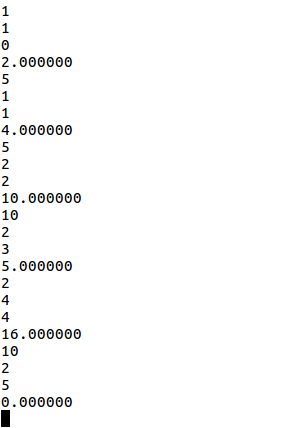
\includegraphics[scale = 0.5]{1.png}
   \caption{Ejecución de la calculadora}
  \end{figure}
  
  Se tiene el siguiente código que halla los primos entre 0 y n.
  
  \begin{lstlisting}
bool esprimo(int num){
	for(int i = num - 1; i > 1){
		if((num % i) == 0){
			return false;
		}
	}i--;
	return true;
}

void primos(int n){
	bool flag;
	for(int i = 1; i <= n){
		flag = esprimo(i);
		if(flag == true){
			print i;
		}
	}i++;
}

int main(){
 	int n;
 	in n;
 	primos(n);
}
  \end{lstlisting}
  
  La tabla de símbolos generada es la siguiente:
  
  \begin{lstlisting}
                 num INT 4 0
                _T0  INT 0 1
                _T1  INT 0 0
                   i INT 4 0
                _T2  INT 0 1
                _T3  BOOL 0 0
                _T4  INT 0 0
                _T5  INT 0 0
                _T6  BOOL 0 0
                _T7  BOOL 0 0
                _T8  INT 0 1
                _T9  BOOL 0 1
                   n INT 8 0
                flag BOOL 8 0
                _T10 INT 0 1
                   i INT 8 0
                _T11 BOOL 0 0
                _T12 BOOL 0 1
                _T13 BOOL 0 0
                _T14 INT 0 1
                   n INT 9 0
                _T15 INT 0 0
  \end{lstlisting}

  La tabla de funciones generada es la siguiente:
  
  \begin{lstlisting}
              global 0
             _F0_FOR 0
          _F1_IF-FOR 0
              _F2_IF 0
             esprimo 260 num 
             _F3_FOR 0
          _F4_IF-FOR 0
              _F5_IF 0
              primos 263 n 
                main 258
  \end{lstlisting}
  
  El código intermedio generado es el siguiente:
  
  \begin{lstlisting}
FUNC esprimo
  RESTAR _T1  num _T0 
  MOVER i _T1 
  FUNC _F1_IF-FOR
    OP_MAYOR _T3  i _T2 
    SALTARV _F0_FOR _T3 
  END
  FUNC _F0_FOR
    OP_MODULO _T4  num i
    OP_IGUALDAD _T6  _T4  _T5 
    FUNC _F2_IF
      INST_RETURN _T7 
    END
    SALTARV _F2_IF _T6 
    RESTAR i i _T8 
    SALTAR _F1_IF-FOR VOID VOID
  END
  SALTAR _F1_IF-FOR VOID VOID
  INST_RETURN _T9 
END
FUNC primos
  MOVER i _T10
  FUNC _F4_IF-FOR
    OP_MENOR_IGUAL _T11 i n
    SALTARV _F3_FOR _T11
  END
  FUNC _F3_FOR
    SALTAR esprimo flag i 
    OP_IGUALDAD _T13 flag _T12
    FUNC _F5_IF
      IMPRIMIR i
    END
    SALTARV _F5_IF _T13
    SUMAR i i _T14
    SALTAR _F4_IF-FOR VOID VOID
  END
  SALTAR _F4_IF-FOR VOID VOID
END
FUNC main
  OP_IN n
  SALTAR primos VOID n 
END
SALTAR main _T15 VOID
  \end{lstlisting}

  Se tiene el siguiente resultado al ejecutar:
  
  \begin{figure}[H]
   \centering
   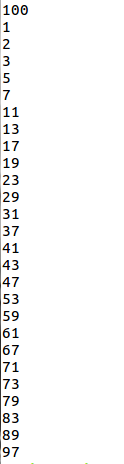
\includegraphics[scale = 0.5]{2.png}
   \caption{Ejecución del buscador de primos}
  \end{figure}



 
\end{enumerate}


\end{document}

